\section{Marco teórico}


Un circuito resonante esta compuesto por una bobina y un capacitor (Figura 1), en el cual se produce una resonancia en una frecuencia determinada. La frecuencia de resonancia es aquella en 
la cual la reactancia inductiva y la reactancia capacitiva son iguales, por lo que la impedancia del circuito es puramente resistiva. 

\begin{figure}[h]
    \centering
    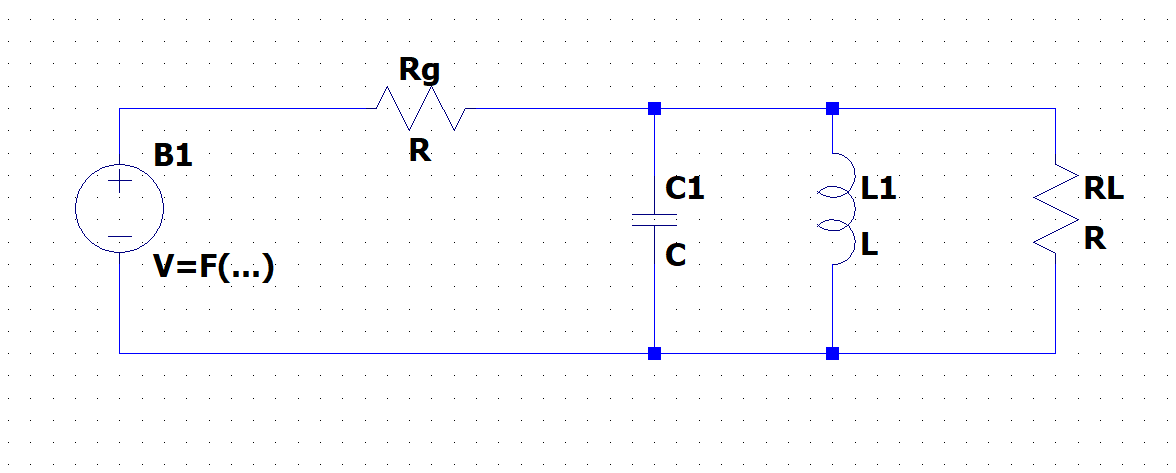
\includegraphics[width=0.5\textwidth]{Imagenes/circuito_resonante.png}
    \caption{Circuito resonante LC}
    \label{fig:circuito_resonante}
\end{figure}

La frecuencia de resonancia o frecuencia central ($f_0$) se calcula mediante la siguiente ecuación:

\begin{equation}
    f_0 = \frac{1}{2\pi \sqrt{LC}}
\end{equation}

A partir de la $f_0$ podemos definir el factor de calidad cuando el circuito esta cargado ($Q_c$) y cuando el circuito esta descargado ($Q_d$). 
Se pueden calcular mediante las siguientes ecuaciones:

\begin{equation}
    Q_c = \frac{f_0}{BW} = \frac{R_T}{X_L}
\end{equation}

\begin{equation}
    Q_d = \frac{R_P}{X_L}
\end{equation}

Donde: 

\begin{itemize}
    \item $R_T$ es la resistencia total
    \item $R_P$ es la resistencia paralelo
    \item $X_L$ es la reactancia inductiva
    \item $BW$ es el ancho de banda
\end{itemize}

$R_T$ define el factor de calidad del circuito cuando esta cargado, y $R_P$ cuando esta descargado.
Y $R_T$ se calcula mediante la siguiente ecuación:

% RT =  RP // RL // Rg
\begin{equation}
    R_T = R_P \parallel R_L \parallel R_g
\end{equation}

%Modificaremos el circuito de la figura 1, para obtener el circuito de acoplamiento interetapas (Figura 2). 
Modificaremos el circuito de la figura 1, para obtener el circuito de acoplamiento interetapas (Figura 2). 

\begin{figure}[h]
    \centering
    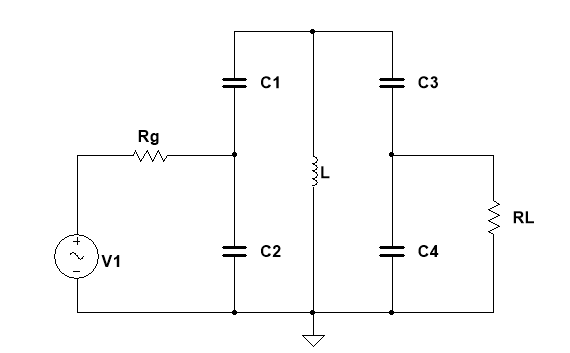
\includegraphics[width=0.5\textwidth]{Imagenes/circuito_acoplamiento2.png}
    \caption{Circuito de acoplamiento interetapas LC modificado}
\end{figure}

El circuito de la figura 2 tiene la misma frecuencia central que el circuito de la figura 1. Si calculamos la capacidad total, obtendremos la misma que la del circuito de la figura 1.

\begin{equation}
    C_T = \frac{C1 \cdot C2}{C1 + C2} + \frac{C3 \cdot C4}{C3 + C4} = \frac{C}{2} + \frac{C}{2} 
\end{equation}

Analizando la salida del circuito de la figura 2, podemos interpretarla como un auto transformador:

\begin{figure}[h]
    \centering
    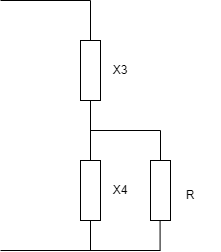
\includegraphics[width=0.3\textwidth]{Imagenes/Esquema_autotrafo.png}
    \caption{Auto transformador}
\end{figure}


Del autotransformador podemos obtener la relación de transformación:

\begin{figure}[h]
    \centering
    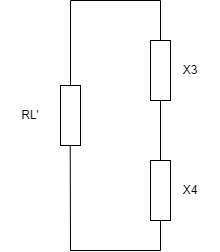
\includegraphics[width=0.3\textwidth]{Imagenes/relacion_transformacion.png}
    \caption{Esquema de relación de transformación}
\end{figure}

% RL prima = (1 + N2/N1)^2 * RL
\begin{equation}
    R_L' = (1 + \frac{X_3}{X_4})^2 \cdot R_L 
\end{equation}


Finalmente, el circuito reflejado de la figura 2 queda como se muestra en la figura 5:

\newpage
\begin{figure}[h]
    \centering
    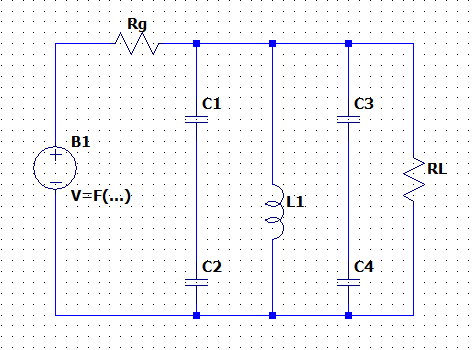
\includegraphics[width=0.5\textwidth]{Imagenes/circuito_reflejado.png}
    \caption{Circuito reflejado}
\end{figure}



Donde nos queda una resistencia total de:

\begin{equation}
    R_T = R_g' \parallel R_L' \parallel R_P
\end{equation}

Donde:

\begin{itemize}
    \item $R_g'$ es la resistencia del generador reflejada
    \item $R_L'$ es la resistencia de carga reflejada
    \item $R_P$ es la resistencia paralelo
\end{itemize}

Podemos realizar la siguiente asignacion de valores, donde seguiremos cumpliendo la condicion de la ecuacion 7:

% RT = Rg' // (RL' // RP)
\begin{equation}
    R_T = X_L \cdot Q_c = R_g' \parallel (R_L' \parallel R_P) = 2 R_T \parallel 2 R_T 
\end{equation}

Retomando el concepto de auto transformador, podemos demostrar que la reflexion de RL y Rg al primario. El procedimiento lo realizaremos solamente con RL, ya que el procedimiento es el mismo para Rg.
Sabemos que la relacion de transformacion en la figura 3 es:

\begin{equation}
    n = \frac{X_3+X_4}{X_4} = 1 + \frac{X_3}{X_4} = \frac{V_{34}}{V_4} = \frac{I_4}{I_{34}}
\end{equation}

Si elevamos al cuadrado la ecuacion 9, obtenemos:

% n^2 = (1 + X3/X4)^2 = V34/V4 * I4/I34
\begin{equation}
    n^2 = (1 + \frac{X_3}{X_4})^2 = \frac{V_{34}}{V_4} \cdot \frac{I_4}{I_{34}} = R_L' / R_L
\end{equation}

Despejando $R_L'$, obtenemos:

% RL' = n^2 * RL
\begin{equation}
    R_L' = n^2 \cdot R_L = (1 + \frac{X_3}{X_4})^2 \cdot R_L = (1 + \frac{C_3}{C_4})^2 \cdot R_L
\end{equation}

Si realizamos el mismo procedimiento con Rg, obtenemos:

% Rg' = n^2 * Rg
\begin{equation}
    R_g' = n^2 \cdot R_g = (1 + \frac{X_1}{X_2})^2 \cdot R_g = (1 + \frac{C_1}{C_2})^2 \cdot R_g
\end{equation}

Finalmente nos quedan 4 ecuaciones con 4 incognitas, las cuales son $C_1$, $C_2$, $C_3$ y $C_4$.
% 4 ecuaciones en una misma llave para que quede mas prolijo y se vea claras las ecuaciones
\begin{equation}
    \begin{cases}
        R_L' = (1 + \frac{C_3}{C_4})^2 \cdot R_L \\
        R_g' = (1 + \frac{C_1}{C_2})^2 \cdot R_g \\
        \frac{ C_1 \cdot C_2}{C_1 + C_2} = \frac{C}{2} \\
        \frac{ C_3 \cdot C_4}{C_3 + C_4} = \frac{C}{2} \\
    \end{cases}
\end{equation}

Con estas ecuaciones podremos comenzar con el calculo para el diseño del circuito de acoplamiento.


